\scanpage{13}
et $(P^\varepsilon)'(\zeta)=N\zeta^{N-1}+(N-1)a_1\zeta^{N-2}+\cdots+a_{N-1}$ soit $\in k^*$ (donc en fait $\in k_0^*$), de sorte qu'il existe une unique $F\in S_n$ telle que $P(F)=0$ et $\varepsilon(F)=\zeta$. Dans ces conditions, on a $F\in A_n$. [En d'autres termes, le couple $(A_n,\mu_n=\mathfrak m_n\cap A_n)$ est (non seulement \unsure{zariskien}, selon le cor. 1, mais même) hensélien]

\deleted{\unsure{Quitte à remplacer} $Z$ par $Z+\zeta$, SPS $\zeta=0$ donc $a_N=\varepsilon(f_N)=0$. En effet, on regarde $X_{n+1}\to X_{n+1}$ donné par
\[
(x_1,\ldots,x_n,x_{n+1})\longmapsto
(x_1,\ldots,x_n,x_{n+1}^{\unsure{N+1|N}}+f_1(x_1,\ldots,x_n)x_{n+1}\cdots)
\]
L'hyp. sur}
\figure{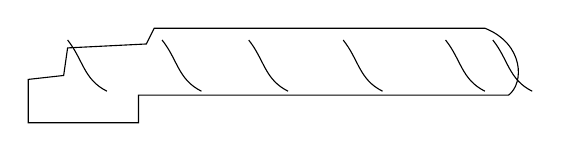
\begin{tikzpicture}[x=1cm,y=1cm]\draw (0,0)--(0,.55)--(.45,.6)--(.5,.95)--(1.5,1)--(1.6,1.2)--(5.8,1.2).. controls (6.3,1) and (6.3,.5)..(6.1,.35)--(1.4,.35)--(1.4,0)--cycle;\foreach \x in {.5,1.7,2.8,4,5.3,5.9}{\draw (\x,1.05) .. controls (\x+.2,.8) and (\x+.2,.55)..(\x+.5,.4);}\end{tikzpicture}}

Plus généralement

\uline{Cor 3} Soit $P\in A_{n+1}[t_1,\ldots,t_n,Z]$, $P=f_0+f_1Z+f_2Z^2+\cdots$ [les $f_i\in S_n(t_1,\ldots,t_n)$] supposons $\varepsilon(f_0)=0$ i.e. $\varepsilon(P)=0$, et $\varepsilon(f_1)\in k^*$ i.e. $\varepsilon\left(\frac{\partial P}{\partial Z}\right)\in k^*$, de sorte qu'il existe une unique $F\in S_n$ telle que $P(t_1,\ldots,t_n,F(t_1,\ldots,t_n))=0$ et $\varepsilon(F)=0$. Alors $F\in A_n$.

Soit en effet $u:X_{n+1}\mathbin{-}X_{n+1}$ donné par
\[
(x_1,\ldots,x_n,\zeta)\longmapsto(x_1,\ldots,x_n,P(x_1,\ldots,x_n,\zeta)),
\]
alors l'hyp. dit que c'est compatible avec les ponctuations, et que c'est un isomorphisme formel. Comme l'hyp. $P\in A_{n+1}$ implique $u$ un $A_*$-morphisme, $\unsure{u'|u^{-1}}$ est un $A_*$ morphisme et par suite $u^{-1}$ est un $A_*$-morphisme. Donc
\[
u^{-1}(x_1,\ldots,x_n,\zeta)=(x_1,\ldots,x_n,\deleted{\unsure{x}}\varphi(x_1,\ldots,x_n,\zeta))
\]
avec $\varphi\in A_{n+1}(t_1,\ldots,t_n,t_{n+1})$, donc $\inserted{F=}\varphi(t_1,\ldots,t_n,0)\in A_n(t_1,\ldots,t_n)$.
\margin{a) b) c) d) impliquent-ils que $S_n$ est fid. plat sur $A_n$ (si $k$ \deleted{\unsure{est}} l'est sur $k_0$)?}

\deleted{\unsure{d)|e)} (Condition différentielle) les $A_n$ sont stables par les opérateurs différentiels standards
\[
D_{\unsure{p_i|\underline p}}=D_{(p_1,\ldots,p_n)}
\left(=\frac{1}{p_1!\cdots p_n!}\frac{\partial^{|p|}}{\partial x_1^{p_1}\cdots\partial x_n^{p_n}}\right).
\]}
\figure{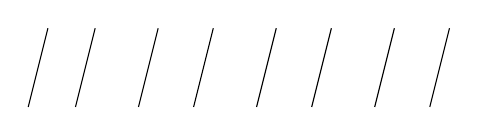
\begin{tikzpicture}[x=1cm,y=1cm]\foreach \x in {0,.6,1.4,2.1,2.9,3.6,4.4,5.1}{\draw (\x,0)--(\x+.25,1);}\end{tikzpicture}}
\mspage{12}
